% Drawing 29/05-1 -- folder 29, batch 05, archive page 87 (PDF page 88).
% Transcription: croquis en marge de gauche : un trait oblique « $D_{o} = X_{o}$ » coupé par deux traits courts épais, « $D_{1}$ » en haut et « $D_{2}$ » en bas ; entre les deux, sur $D_{o}$, une marque épaisse (une petite flèche pointant vers la gauche) et la lettre « $\bar{\xi}_{o}$ ».
% Kind: a divisor D_0 = X_0 cut by D_1 and D_2, with the point xi_0. Method 2 (schematic redraw from the facsimile). Status: partial.
% Notes: The oblique line D_0 = X_0, the two short heavy strokes that cross it (D_1 above, D_2 below), each drawn through a point computed on D_0, the labels where he wrote them, and between the two crossings the point marked on D_0 with the short heavy stroke that ends on it from the right (on the page a small arrow pointing left, towards the line) and the label xi-bar_0. Left out: a faint pencil circle round the marked point and a faint arc at the foot of the crop. Still differs: the heavy mark between the crossings is drawn as a point with a short arrow; on the page it is a blotted arrowhead. Redrawn 2026-11-12 (issue 128): to check again.
% Coordinates: 1 unit = 0.5 mm = 1/100 of the crop width (bbox in page fractions: [0.09, 0.15, 0.27, 0.26]).
% Redrawn by Claude (claude-fable-5-2), issue #128, 2026-11-12; not checked by a human; not compiled (no TeX in the session).
% Rights: reproduces part of the work -- behind RENDER_TRANSCRIPTS, never published by itself.
\documentclass[tikz,border=3pt]{standalone}
\usepackage{amsmath,amssymb}
\usetikzlibrary{patterns,arrows.meta}
\tikzset{pencil/.style={black!45}, struck/.style={black!35}, mpt/.style={circle,draw,inner sep=1.3pt}, pt/.style={circle,fill,inner sep=0.9pt}, opt/.style={circle,draw,fill=white,inner sep=1.1pt}}
\begin{document}
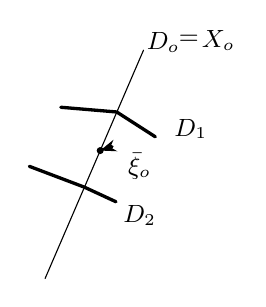
\begin{tikzpicture}[x=0.5mm,y=0.5mm,line cap=round,line join=round,font=\scriptsize]
\draw (58,-17) -- (33,-75);
\draw[very thick] (37,-31.5) -- (51.2,-32.7) -- (61,-39);
\draw[very thick] (29,-46.5) -- (43,-51.8) -- (51,-55.5);
\node[pt] at (47,-42.5) {};
\draw[very thick,-{Stealth[length=2mm]}] (50,-41.5) -- (47,-42.5);
\node[inner sep=1pt] at (63,-15) {\small $D_{o}$};
\node[inner sep=1pt] at (69.5,-14.5) {\small $=$};
\node[inner sep=1pt] at (77,-14.5) {\small $X_{o}$};
\node[inner sep=1pt] at (70,-37) {\small $D_{1}$};
\node[inner sep=1pt] at (57,-59) {\small $D_{2}$};
\node[inner sep=1pt] at (57,-46.5) {\small $\bar{\xi}_{o}$};
\end{tikzpicture}
\end{document}
